\documentclass{standalone}
\usepackage{tikz}
\usetikzlibrary{arrows.meta,positioning,calc}

% Enhanced colors
\definecolor{staticBlue}{RGB}{51, 102, 204}
\definecolor{snapshotCyan}{RGB}{0, 170, 204}
\definecolor{continuousOrange}{RGB}{255, 153, 51}

\begin{document}
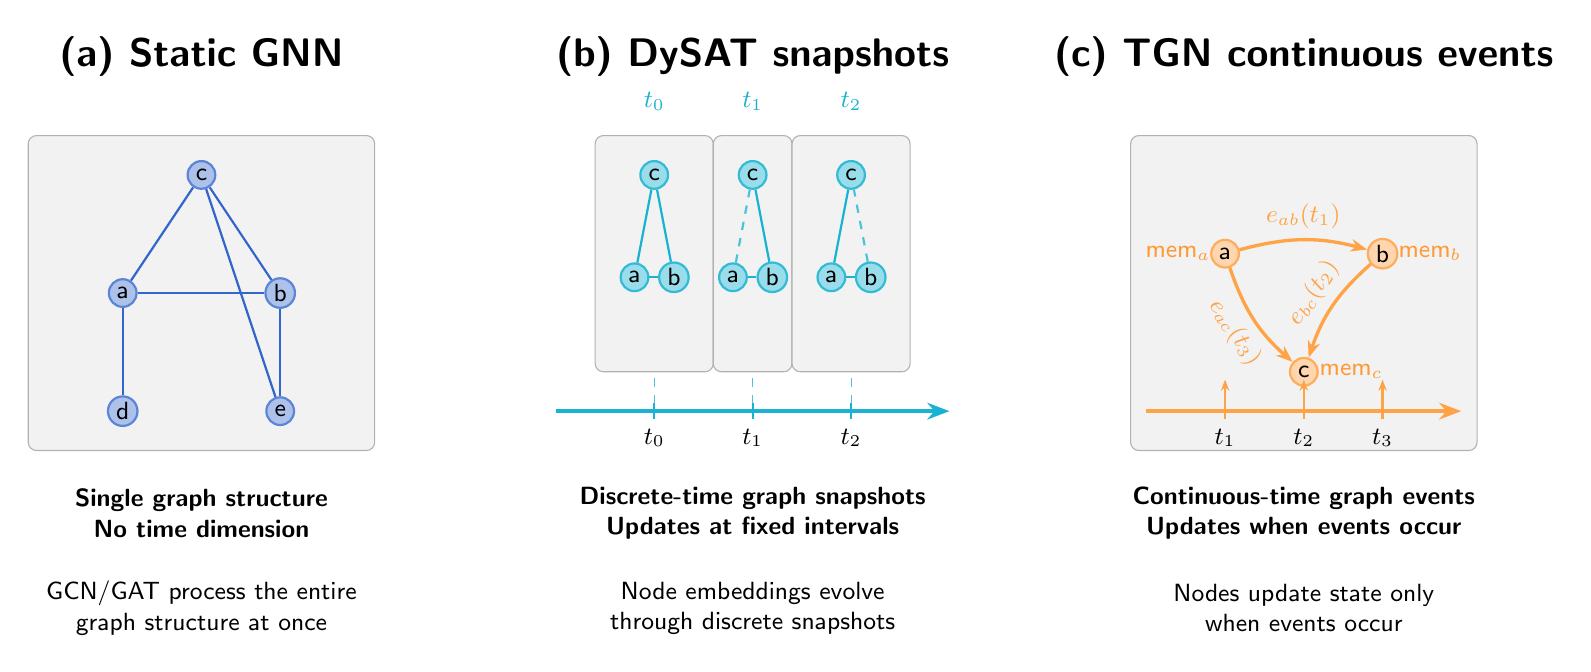
\begin{tikzpicture}[
    % Enhanced styling
    node/.style={circle, draw=black, thick, minimum size=10pt, inner sep=1pt, font=\sffamily\small},
    staticnode/.style={node, fill=staticBlue!40, draw=staticBlue!80},
    dysatnode/.style={node, fill=snapshotCyan!40, draw=snapshotCyan!80},
    tgnnode/.style={node, fill=continuousOrange!40, draw=continuousOrange!80},
    box/.style={draw=black!30, rounded corners=3pt, fill=black!5, inner sep=10pt},
    title/.style={font=\sffamily\Large\bfseries},
    subtitle/.style={font=\sffamily\small\bfseries, align=center},
    note/.style={font=\sffamily\small, align=center}
]

% Fixed positions with better spacing
\def\coldist{7}

%%%%%%%%%%%%%%%%%%%%%%%%%%%%%%%%%%%%%%%%%
% STATIC GNN - COLUMN 1
%%%%%%%%%%%%%%%%%%%%%%%%%%%%%%%%%%%%%%%%%
\node[title] at (0, 4) {(a) Static GNN};

% Static Graph Box
\draw[box] (-2.2, -1) rectangle (2.2, 3);

% Static nodes with better styling
\node[staticnode] (a) at (-1, 1) {a};
\node[staticnode] (b) at (1, 1) {b};
\node[staticnode] (c) at (0, 2.5) {c};
\node[staticnode] (d) at (-1, -0.5) {d};
\node[staticnode] (e) at (1, -0.5) {e};

% Static edges
\draw[staticBlue, thick] (a) -- (b);
\draw[staticBlue, thick] (a) -- (c);
\draw[staticBlue, thick] (b) -- (c);
\draw[staticBlue, thick] (a) -- (d);
\draw[staticBlue, thick] (b) -- (e);
\draw[staticBlue, thick] (c) -- (e);

% Static labels
\node[subtitle] at (0, -1.8) {Single graph structure\\No time dimension};
\node[note] at (0, -3) {GCN/GAT process the entire\\graph structure at once};

%%%%%%%%%%%%%%%%%%%%%%%%%%%%%%%%%%%%%%%%%
% DYSAT - COLUMN 2
%%%%%%%%%%%%%%%%%%%%%%%%%%%%%%%%%%%%%%%%%
\node[title] at (\coldist, 4) {(b) DySAT snapshots};

% Snapshot boxes
\draw[box] (\coldist-2, 0) rectangle (\coldist-0.5, 3); % t0
\draw[box] (\coldist-0.5, 0) rectangle (\coldist+0.5, 3); % t1
\draw[box] (\coldist+0.5, 0) rectangle (\coldist+2, 3); % t2

% Snapshot labels
\node[font=\sffamily\small, snapshotCyan!90, above=0.2cm] at (\coldist-1.25, 3) {$t_0$};
\node[font=\sffamily\small, snapshotCyan!90, above=0.2cm] at (\coldist, 3) {$t_1$};
\node[font=\sffamily\small, snapshotCyan!90, above=0.2cm] at (\coldist+1.25, 3) {$t_2$};

% Snapshot nodes with connections - t0
\node[dysatnode] (c0) at (\coldist-1.25, 2.5) {c};
\node[dysatnode] (a0) at (\coldist-1.5, 1.2) {a};
\node[dysatnode] (b0) at (\coldist-1, 1.2) {b};
% Edges in snapshot t0
\draw[thick, snapshotCyan!90] (a0) -- (b0);
\draw[thick, snapshotCyan!90] (a0) -- (c0);
\draw[thick, snapshotCyan!90] (b0) -- (c0);

% Snapshot nodes with connections - t1
\node[dysatnode] (c1) at (\coldist, 2.5) {c};
\node[dysatnode] (a1) at (\coldist-0.25, 1.2) {a};
\node[dysatnode] (b1) at (\coldist+0.25, 1.2) {b};
% Edges in snapshot t1 - showing evolution
\draw[thick, snapshotCyan!90] (a1) -- (b1);
\draw[thick, snapshotCyan!90] (b1) -- (c1);
\draw[thick, dashed, snapshotCyan!70] (a1) -- (c1); % Changed connection

% Snapshot nodes with connections - t2
\node[dysatnode] (c2) at (\coldist+1.25, 2.5) {c};
\node[dysatnode] (a2) at (\coldist+1, 1.2) {a};
\node[dysatnode] (b2) at (\coldist+1.5, 1.2) {b};
% Edges in snapshot t2 - further evolution
\draw[thick, snapshotCyan!90] (a2) -- (b2);
\draw[thick, dashed, snapshotCyan!70] (b2) -- (c2); % Changed connection
\draw[thick, snapshotCyan!90] (a2) -- (c2); % Connection restored

% Timeline
\draw[ultra thick, -{Stealth[length=8pt]}, snapshotCyan!90] (\coldist-2.5, -0.5) -- (\coldist+2.5, -0.5);

% Timeline ticks
\draw[thick, snapshotCyan!90] (\coldist-1.25, -0.4) -- (\coldist-1.25, -0.6);
\node[font=\sffamily\small, below] at (\coldist-1.25, -0.6) {$t_0$};

\draw[thick, snapshotCyan!90] (\coldist, -0.4) -- (\coldist, -0.6);
\node[font=\sffamily\small, below] at (\coldist, -0.6) {$t_1$};

\draw[thick, snapshotCyan!90] (\coldist+1.25, -0.4) -- (\coldist+1.25, -0.6);
\node[font=\sffamily\small, below] at (\coldist+1.25, -0.6) {$t_2$};

% Connect timeline to snapshots
\draw[dashed, snapshotCyan!70] (\coldist-1.25, -0.4) -- (\coldist-1.25, 0);
\draw[dashed, snapshotCyan!70] (\coldist, -0.4) -- (\coldist, 0);
\draw[dashed, snapshotCyan!70] (\coldist+1.25, -0.4) -- (\coldist+1.25, 0);

% DySAT labels
\node[subtitle] at (\coldist, -1.8) {Discrete-time graph snapshots\\Updates at fixed intervals};
\node[note] at (\coldist, -3) {Node embeddings evolve\\through discrete snapshots};

%%%%%%%%%%%%%%%%%%%%%%%%%%%%%%%%%%%%%%%%%
% TGN - COLUMN 3
%%%%%%%%%%%%%%%%%%%%%%%%%%%%%%%%%%%%%%%%%
\node[title] at (2*\coldist, 4) {(c) TGN continuous events};

% TGN box
\draw[box] (2*\coldist-2.2, -1) rectangle (2*\coldist+2.2, 3);

% TGN nodes with memory - better positioned
\node[tgnnode] (n1) at (2*\coldist-1, 1.5) {a};
\node[font=\sffamily\small, continuousOrange] at (2*\coldist-1.6, 1.5) {mem$_a$};

\node[tgnnode] (n2) at (2*\coldist+1, 1.5) {b};
\node[font=\sffamily\small, continuousOrange] at (2*\coldist+1.6, 1.5) {mem$_b$};

\node[tgnnode] (n3) at (2*\coldist, 0) {c};
\node[font=\sffamily\small, continuousOrange] at (2*\coldist+0.6, 0) {mem$_c$};

% TGN event edges with better styling
\draw[-{Stealth[length=6pt]}, very thick, continuousOrange!90, bend left=15] (n1) to 
    node[midway, sloped, above, font=\small] {$e_{ab}(t_1)$} (n2);
\draw[-{Stealth[length=6pt]}, very thick, continuousOrange!90, bend right=15] (n2) to 
    node[midway, sloped, above, font=\small] {$e_{bc}(t_2)$} (n3);
\draw[-{Stealth[length=6pt]}, very thick, continuousOrange!90, bend right=15] (n1) to 
    node[midway, sloped, below, font=\small] {$e_{ac}(t_3)$} (n3);

% Timeline with better positioning
\draw[ultra thick, -{Stealth[length=8pt]}, continuousOrange!90] (2*\coldist-2, -0.5) -- (2*\coldist+2, -0.5);

% Event markers with better styling
\foreach \x/\t in {-1/1, 0/2, 1/3} {
    \draw[thick, continuousOrange!90] (2*\coldist+\x, -0.4) -- (2*\coldist+\x, -0.6);
    \node[font=\sffamily\small, below] at (2*\coldist+\x, -0.6) {$t_{\t}$};
    \draw[-{Stealth[length=4pt]}, thick, continuousOrange!90] (2*\coldist+\x, -0.4) -- (2*\coldist+\x, -0.1);
}

% TGN labels
\node[subtitle] at (2*\coldist, -1.8) {Continuous-time graph events\\Updates when events occur};
\node[note] at (2*\coldist, -3) {Nodes update state only\\when events occur};

\end{tikzpicture}
\end{document}